\documentclass[a4paper, 12pt, twoside, openright]{book}
\usepackage[english,italian]{babel}
\usepackage[T1]{fontenc}
\usepackage[utf8]{inputenc}
\usepackage{fancyhdr}
\usepackage{float}
\usepackage{graphicx}
\usepackage{wrapfig}
\usepackage{siunitx} %per scrivere il simbolo °
\usepackage{verbatim} %per i commenti1
\usepackage{subfig}
\usepackage{amsmath}
\usepackage{algorithm}
\usepackage{algorithmic}
\setcounter{secnumdepth}{3}
\setcounter{tocdepth}{6}
\usepackage{multirow}
\newcommand{\minitab}[2][l]{\begin{tabular}#1 #2\end{tabular}}
\usepackage{rotating}
\usepackage{xfrac}
\usepackage{enumitem}
\usepackage{amsmath}
%\usepackage{showlabels}
\usepackage{cases}

\DeclareMathOperator*{\argmax}{arg\,max}
\DeclareMathOperator*{\argmin}{arg\,min}

%\usepackage{booktabs,array}
%\usepackage{tikz}

%\usepackage{tabularx}

%\usepackage{chngcntr}
%\counterwithin{table}{section}

%------------------------------ colors
\usepackage[usenames,dvipsnames,table]{xcolor} % use colors on table and more
\definecolor{333}{RGB}{51, 51, 51} % define custom color
\definecolor{background}{RGB}{255, 254, 213}
\definecolor{comment}{RGB}{17,167,5}
\definecolor{keyword}{RGB}{195,47,8}
\definecolor{string}{RGB}{142,195,0}
\definecolor{number}{RGB}{90,84,84}
\definecolor{identifier}{RGB}{0,90,201}

%------------------------------ source code
\usepackage{listings}

\lstset{
  basicstyle=\footnotesize\sffamily,
  commentstyle=\itshape\color{gray},
  captionpos=b,
  frame=shadowbox,
  language=HTML,
  rulesepcolor=\color{333},
  tabsize=2
}

\lstdefinestyle{code}{
  backgroundcolor=\color{background},
  basicstyle=\footnotesize\sffamily,
  commentstyle=\color{comment},
  frame=L,
  identifierstyle=\color{identifier},
  keywordstyle=\color{keyword},
  numbers=left,
  numbersep=10pt,
  numberstyle=\tiny\color{number},
  stringstyle=\color{string},
  showstringspaces=false,  
  stepnumber=1,
  tabsize=2
}


%------------------------------ define Abstract environment, missing in the 'book' class
\newenvironment{abstract}{\cleardoublepage \null \vfill \begin{center}\bfseries\abstractname \end{center}}{\vfill\null}
\addto\captionsenglish{\renewcommand*\abstractname{Abstract}} % change Abstract title

%------------------------------ active url
\usepackage{url}
\renewcommand{\UrlFont}{\color{black}\small\ttfamily}
\usepackage[colorlinks=true, linkcolor=black, citecolor=black, urlcolor=black]{hyperref} % active ref
%------------------------------ macros
\newcommand{\sectionname}{Section} % define Section ref
\newcommand{\subsectionname}{Sub-section} % define Sub-section ref
\renewcommand*\arraystretch{1.4} % tables padding

%acronimi
\usepackage[printonlyused]{acronym}

\begin{document}
\frontmatter

\begin{titlepage} %------------------------------ TITLE PAGE
\begin{center}

\hspace{0.5cm}
\begin{minipage}{.20\textwidth}
  
\includegraphics[height=2.5cm]{Images/UNIPD}
\end{minipage}\begin{minipage}{.90\textwidth}
  \begin{table}[H]
  \begin{tabular}{l}
  \scshape{\Large{\bfseries{Università degli Studi di Padova}}} \\
  \hline \\
  \scshape{\Large{Facoltà di Ingegneria}} \\
  \end{tabular}
  \end{table}
\end{minipage}

\vspace{1cm}
\emph{\Large{Corso~di~Laurea~Magistrale~in~Ingegneria~Informatica}} \\
\vspace{3cm}
\scshape{\Large{Tesina di Ricerca Operativa 2}} \\
\end{center}

\vspace{1cm}
\begin{center}
\scshape{\Large{\bfseries{Travelling Salesman}}}\\
\scshape{\Large{\bfseries{Problem}}}
\end{center}

\vspace{3.5cm}

\begin{center}
\emph{Autori}
\vspace{0.2cm}
\begin{table}[h]
\centering
\begin{tabular}{rl}
\vspace{0.2cm}
{Raffaele Di Nardo Di Maio} & {1204879}\\
{Cristina Fabris} & {1205722}\\
\end{tabular}
\end{table}

\end{center}

\vfill
\begin{center}
\hspace{-0.2cm}
\line(1, 0){360}\\
\textsc{Anno Accademico 2019-2020}
\end{center}
\end{titlepage}

%\begin{comment}
\begingroup %------------------------------ CONTENTS
  \makeatletter
  \let\ps@plain\ps@empty
  \makeatother
  \tableofcontents  
  \clearpage
\endgroup
%\end{comment}

\makeatletter
\def\@makechapterhead#1{%
  \vspace*{50\p@}%
  {\parindent \z@ \raggedright \normalfont
    \vskip 20\p@
    \interlinepenalty\@M
    \Huge \bfseries #1\par\nobreak
    \vskip 40\p@
  }}
\makeatother


\mainmatter
\chapter{Introduzione}\label{intro}
La seguente trattazione analizza il Problema del Commesso Viaggiatore (Travelling Salesman Problem, TSP), che consiste nell'individuare un circuito hamiltoniano di costo minimo in un assegnato grafo orientato G=(V,A)\cite{TSP}. La formulazione matematica di tale problema è la seguente:
$$
x_{ij}=
\begin{cases}
1 & se\;l'arco\;(i,j)\in A\;viene\;scelto\;nel\;circuito\;ottimo\\
0 & altrimenti\\
\end{cases}
$$
\begin{align}
& min \underset{(i,j)\in A}\sum{c_{ij}\;x_{ij}} \\\notag \\
& \underset{(i,j)\in \delta^{-}(j)}\sum{\;x_{ij}} = 1 & \forall\;j\in V \\\notag \\
& \underset{(i,j)\in \delta^{+}(i)}\sum{\;x_{ij}} = 1 & \forall\;i\in V \\\notag \\
& \underset{(i,j)\in \delta^{+}(S)}\sum{\;x_{ij}} \geq 1 & S \subset V\; :\; 1\in S\\\notag \\
& x_{ij}\geq 0\;\; intero & (i,j)\in A.\\\notag
\end{align}
Tuttavia le soluzioni algoritmiche presentante risolvono una sua variante, detta simmetrica, che viene applicata ad un grafo completo non orientato G=(V,E).\\ Di seguito viene riportata la formulazione matematica di tale versione:\\
\begin{align}
& min \underset{e\in E}\sum{c_e\;x_e}\\
& \underset{e\in \delta(v)}\sum{\;x_e} = 2 & \forall\;v\in V \\
& \underset{e\in E(S)}\sum{\;x_e} \leq \vert S\vert - 1 & \forall\;S\underset{\neq} \subset V: \vert S\vert\geq 3.\\\notag
\end{align}
A livello commerciale esistono diverse tipologie di risolutori di problemi di programmazione lineare intera, basati sul Branch \& Bound. I più conosciuti in circolazione sono i seguenti:
\begin{itemize}
\item{\textbf{IBM ILOG CPLEX Optimization Studio}\cite{ILOG}\\
è un soluzione analitica, sviluppata dall'IBM e gratuita a livello accademico.}
\item{\textbf{FICO® Xpress Optimization}\cite{FICO}\\
è stato prodotto dalla Fair Isaac Corporation(FICO) ed è costituito da 4 componenti principali: FICO® Xpress Insight, FICO® Xpress Executor, FICO® Xpress Solver e FICO® Xpress Workbench. Questa soluzione è disponibile gratuitamente solo nella versione Community, in cui però vengono applicate restrizioni sul numero di righe e colonne del tableau, di token non lineari e di funzioni dell'utente.}
\item{\textbf{Gurobi}\cite{GUROBI}\\
è una soluzione, sviluppata dalla Gurobi Optimization, che viene rilasciata anche con una versione accademica.}
\item{\textbf{COIN Branch and Cut solver (CBC)}\cite{CBC}\\
è un risolutore MIP(mixed-integer program) open-source scritto in C++ e sviluppato dalla Computational Infrastructure for Operations Researc (COIN).}
\end{itemize}
Nel Capitolo \ref{CPLEX} vengono riportate diverse soluzioni mat-euristiche e non per il problema del Commesso Viaggiatore, che fanno uso di ILOG CPLEX.\\
In commercio, il più noto ed efficiente software per la risoluzione del TSP è Concorde, sviluppato in ANSI C e disponibile per l'uso in ambito accademico\cite{concorde}.\\
Nel Capitolo \ref{HEURISTIC} vengono analizzati gli algoritmi euristici, sviluppati senza far uso di ILOG CPLEX.\\
Nel Capitolo \ref{PERF_PROF} vengono invece riportati i confronti, a livello temporale e di costo, delle soluzioni ottenute con i differenti algoritmi enunciati.\\
Nell'Appendice \ref{TSPlib}, \ref{CPLEX_func}, \ref{gnuplot}, \ref{perf_profile_py} vengono descritte rispettivamente la tipologia di istanze utilizzate, la documentazione utilizzata ed il funzionamento di CPLEX, il programma GNUPLOT utilizzato nella stampa delle soluzioni e il programma perfprof.py usato per creare i performance profile del Capitolo \ref{PERF_PROF}.\\
Tutti i tempi di esecuzione e i costi delle soluzioni, ottenuti mediante la fase di testing, sono consultabili invece nelle tabelle riportate nell'Appendice \ref{results}. Tutte le soluzioni descritte sono state implementate in linguaggio C e testate sul sistema operativo Windows 10 con Visual Studio, ed i sorgenti sono disponibili online\footnote{\url{https://github.com/RaffaDNDM/Operational-Research-2}}.
\chapter{Istanze e soluzioni del problema}
\section{Istanze}
Le istanze del problema, analizzate durante il corso, sono punti dello spazio 2D, identificati quindi da due coordinate ($x$,$y$).
Per generare istanza enormi del problema, si utilizza un approccio particolare in cui viene definito un insieme di punti a partire da un'immagine già esistente.\\
La vicinanza dei punti generati dipende dalla scala di grigi all'interno dell'immagine (es. generazione di punti a partire dal dipinto della Gioconda\cite{monnalisa}).\\
Le istanze che vengono elaborate dai programmi, creati durante il corso, utilizzano il template \textbf{TSPlib}. Di seguito viene riportato il contenuto di un file di questa tipologia.
 
\lstinputlisting[caption={\footnotesize{esempio.tsp}}, style=code, firstnumber=1, firstline=1, lastline=12, label=tsp_instance]{Source/esempio.tsp}

Le parole chiave più importanti, contenute in questi file \ref{tsp_instance}, sono:
\begin{itemize}
\item{\textbf{NAME}\\
seguito dal nome dell'istanza TSPlib}
\item{\textbf{COMMENT}\\
seguito da un commento associato all'istanza}
\item{\textbf{TYPE}\\
seguito dalla tipologia dell'istanza}
\item{\textbf{DIMENSION}\\
seguito dal numero di nodi nel grafo ($num\_nodi$)}
\item{\textbf{EDGE\_WEIGHT\_TYPE}\\
seguito dalla specifica del tipo di calcolo che viene effettuato per ricavare il costo del tour}
\item{\textbf{NODE\_COORD\_SECTION}\\
inizio della sezione composta di $num\_nodi$ righe in cui vengono riportate le caratteriste di ciascun nodo, nella forma seguente:
\begin{lstlisting}[linewidth=250pt,basicstyle=\footnotesize\sffamily,]     
indice_nodo  coordinata_x  coordinata_y
\end{lstlisting}}
\item{\textbf{EOF}\\
decreta la fine del file}
\end{itemize}

\section{Soluzioni}
Una soluzione del problema è una sequenza di nodi che corrisponde ad una permutazione dell'istanza (es. $S = \{x_1,x_2,...,x_n\}$ tale che $x_i=x_j\;\;x_i \in \Pi\;\forall\;x_i\in S\;\wedge\; x_i!=x_j\;\forall\;i\neq j$). Poichè in questa variante non esiste alcuna origine, ogni tour può essere descritto da due versi di percorrenza e l'origine può essere un nodo qualsiasi del grafo.
\subsection{Gnuplot}\label{gnuplot}
Una volta ottenuta la soluzione del problema di ottimizzazione, viene disegnato il grafo per facilitare all'utente la comprensione della sua correttezza. Per fare ciò viene utilizzato Gnuplot, un programma di tipo command-driven.\\
Per poterlo utilizzare all'interno del proprio programma esistono due metodi:
\begin{itemize}
\item{Collegare la libreria ed invocare le sue funzioni all'interno del nostro programma}
\item{Collegare l'eseguibile interattivo al proprio programma. In questo caso i comandi deve essere passati all'eseguibile attraverso un file di testo e l'utilizzo di un pipe.}\\
\end{itemize}
In questa trattazione è stato scelto il secondo metodo. All'interno del file è possibile specificare a Gnuplot le caratteristiche grafiche che deve aver il grafo. Di seguito viene riportato un esempio di tale file.\\

\lstinputlisting[caption={\footnotesize{style.txt}}, style=code, firstnumber=1, firstline=1, lastline=12, label=style_example]{Source/style_example.txt}

Nell'esempio sopra riportato, nella prima parte viene definito lo stile, il colore delle linee e la tipologia di punti, che verrano in seguito visualizzati all'interno del grafico prodotto.\\In seguito viene effettuato il plot del grafo in una finestra, utilizzando il primo e secondo valore di ciascuna riga del file \textbf{solution.dat} come coordinate mentre il terzo valore viene utilizzato come etichetta.\\\\
Il file \textbf{solution.dat} contiene le informazioni relative alla soluzione del grafico in cui ciascuna riga ha la seguente forma:
\begin{lstlisting}[linewidth=290pt,basicstyle=\footnotesize\sffamily,]     
coordinata_x   coordinata_y   posizione_in_tour
\end{lstlisting}
\textbf{coordinata\_x} rappresenta la coordinata x del nodo;\\
\textbf{posizione\_in\_tour} rappresenta la coordinata y del nodo;\\
\textbf{posizione\_in\_tour} rappresenta l'ordine del nodo all'interno del tour, assunto come nodo di origine il nodo 1.\\\\
Il grafico viene generato dal comando \textbf{plot}, leggendo tutte le righe non vuote e disegnando un punto nella posizione \textbf{(coordinata\_x,coordinata\_y)} del grafico 2D. In seguito viene tracciata una linea solo tra coppie di punti, legati a righe consecutive non vuote all'interno di \textbf{solution.dat}.\\\\
Attraverso le istruzioni riportate nelle righe 10-12 di \textbf{style.txt}, viene invece salvato il grafico appena generato nell'immagine \textbf{solution.png}.\\\\
Di seguito vengono riportate le varie fasi necessarie alla definizione di un pipe e al passaggio di questo al programma GNUplot:
\begin{itemize}
\item{\textbf{Definizione del pipe}
\lstinputlisting[style=code, firstnumber=1, firstline=1, lastline=1, label=style_example language=C]{Source/gnuplotC.txt}
dove \textbf{GNUPLOT\_EXE} è una stringa composta dal percorso completo dell'eseguibile di GNUplot, seguita dall'argomento \textbf{-persistent} (es. \textit{"D:/Programs/GNUplot/bin/gnuplot -persistent"}).
}
\item{\textbf{Passaggio delle istruzioni a GNUplot}
\lstinputlisting[style=code, firstnumber=2, firstline=2, lastline=10, label=style_example, language=C]{Source/gnuplotC.txt}
viene passata una riga alla volta, del file \textbf{style.txt}, a GNUplot mediante il pipe precedentemente creato.
}
\item{\textbf{Chiusura del pipe}
\lstinputlisting[style=code, firstnumber=11, firstline=11, lastline=11, label=style_example, language=C]{Source/gnuplotC.txt}
}
\end{itemize}
\chapter{Risoluzione del problema}
Per poter utilizzare gli algoritmi di risoluzione forniti da CPLEX è necessario costruire il modello matematico del problema, legato all'istanza precedentemente descritta.\\
CPLEX ha due meccanismi di acquisizione dell'istanza:
\begin{enumerate}
\item{\textbf{modalità interattiva:}\\
in cui il modello viene letto da un file precedentemente generato (\textit{model.lp})}
\item{\textbf{creazione nel programma:}\\
il modello viene creato attraverso le API del linguaggio usato per la scrittura del programma}
\end{enumerate}

Le strutture utilizzate da CPLEX sono due (vedi Figura \ref{strutture_cplex}):
\begin{itemize}
\item{\textbf{ENV (enviroment):} contiene i parametri necessari all'esecuzione e al salvataggio dei risultati}
\item{\textbf{LP:} contiene il modello che viene analizzato da CPLEX durante la computazione del problema di ottimizzazione}
\end{itemize}

\begin{figure}[h] 
\begin{center} 
  % Requires \usepackage{graphicx} 
  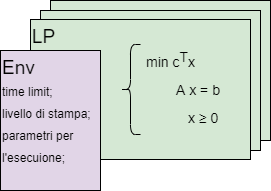
\includegraphics[scale=0.7]{Images/cplex_structs}\\ 
  \caption{\footnotesize{Strutture CPLEX}}
  \label{strutture_cplex} 
\end{center} 
\end{figure}

Ad ogni ENV è possibile associare più LP, in modo da poter risolvere in parallelo più problemi di ottimizzazione, ma nel nostro caso ne sarà sufficiente solo uno.\\
Per convenzione è stato deciso di etichettare i rami $(i,j)$ dell'istanza rispettando la proprietà $i<j$. In Figura \ref{Indici_matrice} è riportato lo schema degli indici che vengono utilizzati per etichettare le variabili.\\
In questa figura le celle $(i,j)$ bianche, sono quelle effettivamente utilizzate per indicare un arco secondo la convenzione. Il numero all'interno di queste caselle rappresenta invece l'ordine in cui queste variabili vengono inserite nel modello e quindi gli indici associati da CPLEX per accedere alla soluzione.
\begin{figure}[h] 
\begin{center} 
  % Requires \usepackage{graphicx} 
  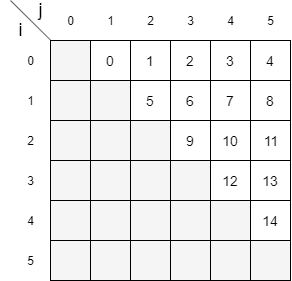
\includegraphics[width=5cm]{Images/indices_matrix}\\ 
  \caption{\footnotesize{Indici della matrice}}
  \label{Indici_matrice} 
\end{center} 
\end{figure}
Il modello così strutturato richiede però l'inserimento di un esponenziale numero di vincoli per l'eliminazione dei sub-tour, vengono quindi ora descritti altri modelli che ovvino a questo problema.\\  

\section{Modelli compatti}
I modelli compatti del Travelling Salesman Problem, sono formulazioni il cui numero di variabili e di vincoli è polinomiale nella taglia dell'istanza. In particolare, in quelle analizzate in seguito, sono entrambi $O(n^2)$, con \textit{n = numero di nodi}.\\
I modelli compatti sono però applicabili solo a grafi orientati. Per poterli sfruttare per la risoluzione del TSP simmetrico, è necessario per ogni ramo dell'istanza $(i,j)$, inserire nel modello i corrispondenti rami orientati in entrambe le direzioni $(i,j)$ e $(j,i)$. Questo comporta un significativo rallentamento nella computazione della soluzione, in quanto l'algoritmo, ogni volta che scarta un ramo $(i,j)$ dalla soluzione ottima, verifica se il corrispondente $(j,i)$ potrebbe invece appartenerle. Questo non può però essere possibile, essendo i due rami in realtà lo stesso nella nostra istanza iniziale.\\ 
\subsection{Formulazione sequenziale}
Miller, Tucker e Zemlin, nella loro formulazione del modello, hanno introdotto una nuova variabile $u_i$ per ogni nodo \textit{i} e imposto che, nella soluzione ottima, il suo valore  rispettasse dei nuovi vincoli. Questi servivano a garantire che venisse seguito un ordine di percorrenza di tutti i nodi. In questo modo hanno eliminato la creazione di sub-tour, mantenendo il numero di vincoli e di variabili polinomiale. Nello specifico il loro modello è così strutturato:
\begin{align}
& min \underset{i\in V}\sum{}\underset{j\in V}\sum{c_{i,j}\; x_{i,j}} \\ \notag \\
& \underset{i\in V}\sum{x_{ih}}\; =\; 1 & \forall\; h\in V \\ \notag \\
& \underset{j\in V}\sum{x_{hj}}\; =\; 1 & \forall\; h\in V \\ \notag \\
& u_i-u_j+n\; x_{i,j}\;\leq\; n-1 & \forall\; i,j\in V-\{ 1\} , i\neq j \\ \notag \\
& 0\leq u_i\;\leq\; n-2 & \forall\; i\in V-\{ 1\} \\ \notag 
\end{align}
Esistono due diversi modi per implementare questo modello sfruttando le funzioni di CPLEX.\\
Nel primo i nuovi vincoli vengono aggiunti come visto in precedenza. In questo modo, durante la fase di preprocessamento, il programma è già a conoscenza di tutti i vincoli che dovrà rispettare la soluzione ottima. Ciò gli permette di migliorare i coefficienti presenti, prima ancora di iniziare la computazione dell'ottimo.\\
Il secondo metodo, invece, sfrutta l'inserimento nel modello di vincoli detti "lazy constraints". Questi non sono noti al programma dall'inizio, ma vengono inseriti all'interno di un pool di vincoli. Nel momento in cui viene calcolata una soluzione, CPLEX verifica che vengano rispettati tutti i vincoli presenti nel pool. Se ne trova uno violato lo aggiunge al modello e ripete la computazione. Questo approccio permette, per risolvere lo stesso problema, di eseguire calcoli su un modello più piccolo, ma può aumentare i tempi di computazione non fornendo a CPLEX tutte le informazioni dall'inizio.   

\subsection{Formulazione basata sul flusso}
Nella formulazione di Gavish e Graves, per impedire la formazione di sub-tour all'interno della soluzione ottima, viene introdotto un nuovo vincolo per ogni ramo del grafo. Questo permette di regolare il flusso $y_{i,j}$, con $i\neq j$,  che lo attraversa.Inoltre è stato necessario aggiungere anche dei vincoli, detti "vincoli di accoppiamento", che collegassero i flussi alle variabili $x_{i,j}$ . Il loro modello è quindi così strutturato:
\begin{align}
& min\underset{i\in V}\sum{\underset{j\in V}\sum{c_{i,j}\; x_{i,j}}} \\ \notag \\
& \underset{i\in V}\sum{x_{ih}}\;=\;1 & \forall\;h\in V \\ \notag\\
& \underset{j\in V}\sum{x_{hj}}\;=\;1 & \forall\;h\in V \\ \notag\\
& \underset{j\in V}\sum{y_{1,j}}\;=\;1\\ \notag\\
& \underset{j\in V}\sum{y_{h,j}}\;=\;\underset{i\in V}\sum{y_{i,h}}\;-1 & \forall\;h\in V-\{1\}\\ \notag\\
& y_{i,j}\leq\;(n-1)\;x_{i,j} & \forall\;i,j\in V, i\neq j\\ \notag
\end{align}
La soluzione di questo modello risulta però essere lontana dalla convex hull. Per migliorarla è possibile sostituire il vincolo \textit{(3.11)} con \\
\begin{center}
$y_{i,j}\leq\;(n-2)\;x_{i,j} \;\;\;\;\;\forall\; i\neq \; j$\\
\end{center}
mentre per gli altri valori di $i$ e $j$ è necessario lasciare i vincoli originali. 
Per evitare che la soluzione ottima contenga sia l'arco $x_{i,j}$ che $x_{j,i}$, che nella nostra istanza iniziale corrispondono allo stesso arco, viene anche aggiunto il seguente vincolo:
\begin{center}
$x_{i,j}+x_{j,i}\leq 1\;\;\;\; \forall i,j \in V$ con $i < j$
\end{center}

\section{Loop}
Negli anni '60, Jacques F. Benders sviluppò un approccio generale, applicabile a qualsiasi problema di programmazione lineare, per ridurre il numero esponenziale di alcuni vincoli specifici inseriti nel modello.\\
Utilizzando questo metodo, il modello viene scritto senza quei vincoli e poi questi verranno aggiunti in seguito durante la risoluzione del problema. Nel caso in cui la soluzione ottima, calcolata a partire da questo modello, non rispetti un vincolo di quelli rimossi, viene aggiunto al modello. \\
Nella seguente parte, viene riportata l'appicazione specifica di loop al problema TSP.
I vincoli di Subtour Elimination sono in numero esponenziale e sono:\\
\begin{align}
&\underset{e\in E(S)}\sum{x_{e}} \leq \mid S\mid - 1\;\forall\;S\underset{\neq}{\subset}V\; : \; \mid S\mid\geq 2
\end{align}
o equivalentemente:
\begin{align}
&\underset{e\in \delta(S)}\sum{x_{e}}\geq 2\;\forall\;S\underset{\neq}{\subset}V\; : \; \mid S\mid\geq 2
\end{align}
Viene definito un nuovo modello per il problema del commesso viaggiatore simmetrico, in cui vengono rimossi tali vincoli, aggiungendo così la possibilità di avere dei subtour nella soluzione finale.\\
Viene risolto il problema e nel caso in cui ci sia più di una componente connessa, viene aggiunto al modello un vincolo di subtour elimination per ogni ciclo generato.\\
\begin{algorithm}
\caption{Risoluzione del problema}
\begin{algorithmic}
\REQUIRE {$MODEL =$ Modello TSP simmetrico senza vincoli di Subtour elimination}
\ENSURE {$x$: soluzione intera senza subtour}
\STATE {}
\STATE {$x \leftarrow solve(MODEL)$}
\STATE {$num\_comps \leftarrow comps(x)$}
\STATE {}
\WHILE{$num\_comps \geq 2$}
\STATE{Add $\underset{e\in \delta(S_k)}\sum{x_{e}}\leq \mid S_k\mid - 1\;\forall\; componente\; connessa\; S_k$}
\STATE {}
\IF{$num\_comps \geq 2$}
\STATE {$x \leftarrow solve(MODEL)$}
\STATE {$num\_comps \leftarrow comps(x)$}
\ENDIF
\STATE {}
\ENDWHILE
\end{algorithmic}
\end{algorithm}
\vspace{10cm}
All'aumentare del numero di vincoli, il costo della soluzione ottenuta da CPLEX peggiora o resta identica a quella elaborata all'iterazione precedente del metodo loop.\\
Il numero di iterazioni che vengono effettuate dall'algoritmo non è conosciuto e potrebbe essere anche molto elevato. Nel caso peggiore vengono inseriti tutti i vincoli di Subtour elimnation, ovvero un numero esponenziale di disequazioni, soprattutto con istanze clusterizzate.\\
Inoltre il problema principale di questo algoritmo è la generazione, ad ogni iterazione, di un albero completo di branching, eliminando quello precedente sviluppato.\\
In passato, con le versioni del MIP solver di CPLEX degli anni '60, questa operazione era molto onerosa mentre attualmente il metodo loop garantisce la risoluzione, anche di istanze molto grandi, in tempi ragionevoli.
Questo non accade invece per il Branch \& Bound in quanto vengono aggiunte nuove ramificazioni all'albero già esistente.\\
L'introduzione di nuovi vincoli di Subtour Elimination, solo nel momento in cui si presenta una loro violazione, permette di ridurre la dimensione del modello ma riduce l'attività di pre-processamento svolta da CPLEX prima di cominciare la risoluzione del problema. Nella fase di pre-processing infatti, vengono applicati algoritmi euristici e cambiamenti dei coefficenti nel modello, in base ai vincoli inseriti.\\
L'algoritmo può essere modificato svolgendo prima il metodo loop con l'aggiunta di parametri differenti da quelli utilizzati di default del risolutore CPLEX. In seguito viene effettuato nuovamente l'algoritmo di Benders ma questa volta nella sua versione esatta, in modo da migliorare la soluzione meta-euristica trovata nella prima parte. \\
Quest'ottimizzazione è basata sul fatto che CPLEX salvi alcune soluzioni, ottenute in precedenza dal risolutore sullo stesso modello, e le sfrutti come bound nel nuovo modello. Per questo motivo, alcune delle soluzioni metaeuristiche ottenute nella prima fase vengono sfruttate come bound nella seconda.
\chapter{Performance}\label{PERF_PROF}
Le metriche di confronto, utilizzate nell'analisi degli algoritmi, sono il tempo complessivo di creazione e risoluzione del modello ed il costo della soluzione ottenuta. Ciascuna modalità di risoluzione viene applicata a diverse istanze di TSPlib, con un numero differente di nodi.  
\section{Performance variabilty}
Nel corso degli anni '90, gli ingegneri di CPLEX scoprirono che il tempo di risoluzione variasse significativamente in diversi sistemi operativi. Con alcune istanze, le performance migliori si avevano su UNIX mentre con altre su Windows.\\
Il motivo di tale comportamento venne in seguito studiato ed attribuito alla diversa scelta effettuata dai sistemi operativi nel decretare l'ordine delle variabili su cui viene svolto l'albero decisionale.\\
Le scelte svolte inizialmente, nella definizione dei primi nodi dell'albero, si ripercuotono sulla sua successiva evoluzione.\\
Proprio per questo motivo, su alcune istanze, UNIX riusciva a risolvere il problema in tempo minore rispetto a Windows, mentre su altre accadeva l'opposto.\\
Da questi studi, evinse che il Branch and Cut è un sistema caotico e che quindi piccole variazioni delle condizioni iniziali generano grandi differenze nei risultati finali.\\
Per questo motivo, alcuni algoritmi prensentati in questo report, sono stati studiati al variare di alcune condizioni iniziali:
\begin{itemize}
\item{\textbf{Random Seed}\\
definisce il seme da cui CPLEX genera una sequenza di numeri pseudo-casuali (vedi Sezione \ref{param}). Nel momento in cui CPLEX nota che diverse variabili frazionarie hanno lo stesso valore, il risolutore sceglie casualmente su quale di queste applicare il Branch.}
\item{\textbf{Gap}\\
intervallo massimo, tra il valore della migliore funzione obiettivo intera e il valore della funzione di costo del miglior nodo rimanente, che permette di decretare il raggiungimento dell'ottimo secondo CPLEX (vedi Sezione \ref{param}).}
\end{itemize}
La variazione del primo di questi parametri permette di apportare significative modifiche al tempo di risoluzione, non modficando la reale ottimalità della soluzione.\\
La variazione dell'altro parametro permette invece di ottenere una soluzione euristica, ovvero un'approssimazione più lasca di quella ottima.
 
\section{Analisi tabulare}
Un metodo non molto efficiente per lo studio delle performance degli algoritmi, utilizza una struttura tabulare in cui viene inserita una riga per ogni istanza del problema.\\ Inoltre vengono riportati i tempi di esecuzione degli algoritmi su ognuno dei grafi analizzati. Nell'ultima riga per ciascun algoritmo viene riportata la media geometrica dei suoi tempi di esecuzione (vedi esempio in Tabella \ref{result_table}).\\
Solitamente viene impostato un TIME LIMIT uguale per tutti gli algoritmi. Questo rappresenta nella tabella il valore del tempo di esecuzione per un algoritmo che ha impiegato un tempo maggiore o uguale a TIME LIMIT. Spesso viene dato più peso al TIME LIMIT, inserendolo nella tabella con, ad esempio, peso 10 (ovvero TIME LIMIT*10).\\ La debolezza di tale calcolo delle performance risiede nel fatto che non sempre la media descrive  l'efficienza di un soluzione. Infatti non influisce unicamente il tempo di risoluzione del modello ma anche quello necessario alla sua creazione. 

\begin{table}[h]
\centering
\begin{tabular}{|c|c|c|c|}
\multicolumn{1}{c}{\textbf{Istanza}} & \multicolumn{1}{c}{\textbf{Sequential}} & \multicolumn{1}{c}{\textbf{Flow}} &
\multicolumn{1}{c}{\textbf{Loop}}\\
\hline
\textbf{att48} & {212.3} & {12.5} & {4.3}\\
\hline
{\textbf{...}} & {...} & {...} & {...}\\
\hline
\textbf{a280} & {3200} & {2500.8} & {1300.5}\\
\hline
\hline
\multicolumn{1}{c}{} & \multicolumn{1}{c}{2120.3} & \multicolumn{1}{c}{1800.3}& \multicolumn{1}{c}{1000.4}\\
\end{tabular}
\caption{\footnotesize{Tabella di performance con \textbf{TIME LIMIT=3200}.}}\label{result_table}
\end{table}

\section{Performance profiling}
Questo metodo prevede la classificazione dei tempi di esecuzione degli algoritmi in base al numero percentuale di successi, rispetto a un fattore moltiplicativo (ratio) del tempo di esecuzione (vedi Figura \ref{perf_profile}).\\
L'andamento del performance profile di un algoritmo è monotono crescente. Il valore assunto per ogni ratio dagli algoritmi all'interno del grafico è la percentuale del numero di istanze che l'algoritmo risolve con quel fattore rispetto all'ottimo di quel caso.\\
Spesso questi grafici vengono rappresentati in scala logaritmica per notare al meglio le differenze ed avere una migliore raffigurazione.\\
\begin{figure}[h] 
\begin{center} 
  % Requires \usepackage{graphicx} 
  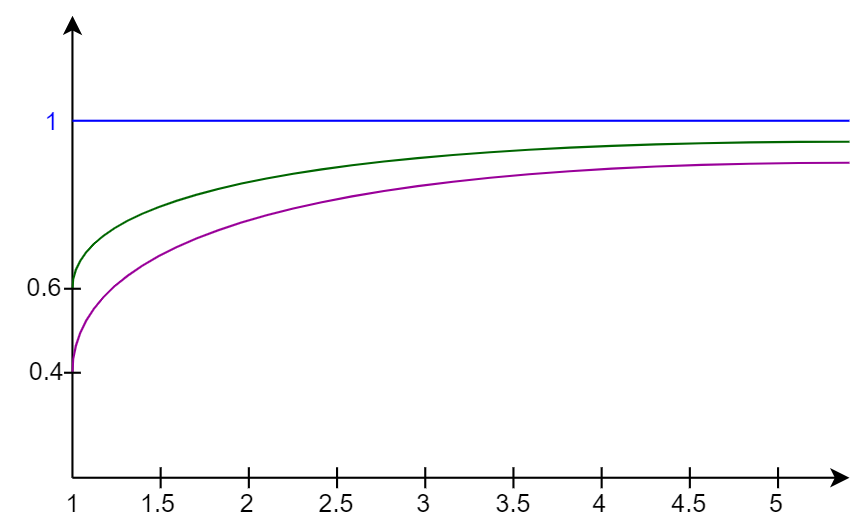
\includegraphics[scale=0.3]{Images/perf_profile} 
  \caption{\footnotesize{Performance profile di due algoritmi.}}
  \label{perf_profile} 
\end{center} 
\end{figure}
Per creare il performance profile degli algoritmi implementati, è stato utilizzato il programma python riportato nella Sezione \ref{perf_profile_py}. 

\section{Analisi degli algoritmi sviluppati}
Nella seguente sezione vengono riportati i grafici relativi ai risultati ottenuti con le implementazioni degli algoritmi descritti nei precedenti capitoli. I valori ottenuti ed utilizzati per realizzare le immagini contenute in questa sezione, sono consultabili nell'Appendice \ref{results}.
\subsection{Algoritmi esatti}
Gli algoritmi basati sul modello compatto, sono stati testati con un time limit di 20 minuti sulle seguenti istanze:
\begin{center}
\begin{multicols}{3}
\begin{itemize}
\item{att48.tsp}
\item{berlin52.tsp}
\item{burma14.tsp}
\item{eil101.tsp}
\item{eil51.tsp}
\item{eil76.tsp}
\item{gr96.tsp}
\item{kroA100.tsp}
\item{kroB100.tsp}
\item{kroB150.tsp}
\item{kroC100.tsp}
\item{kroD100.tsp}
\item{kroE100.tsp}
\item{pr124.tsp}
\item{pr136.tsp}
\item{pr76.tsp}
\item{rat99.tsp}
\item{rd100.tsp}
\item{st70.tsp}
\item{ulysses16.tsp}
\end{itemize}
\end{multicols}
\end{center}
Visionando il performance profile in Figura \ref{pp_compact}, risulta evidente come l'aggiunta dei vincoli come lazy constraint, nel metodo di Miller, Tucker e Zemlin, garantisca un notevole miglioramento delle prestazioni rispetto alla versione originale.\\
\begin{figure}[H] 
\begin{center} 
  % Requires \usepackage{graphicx} 
  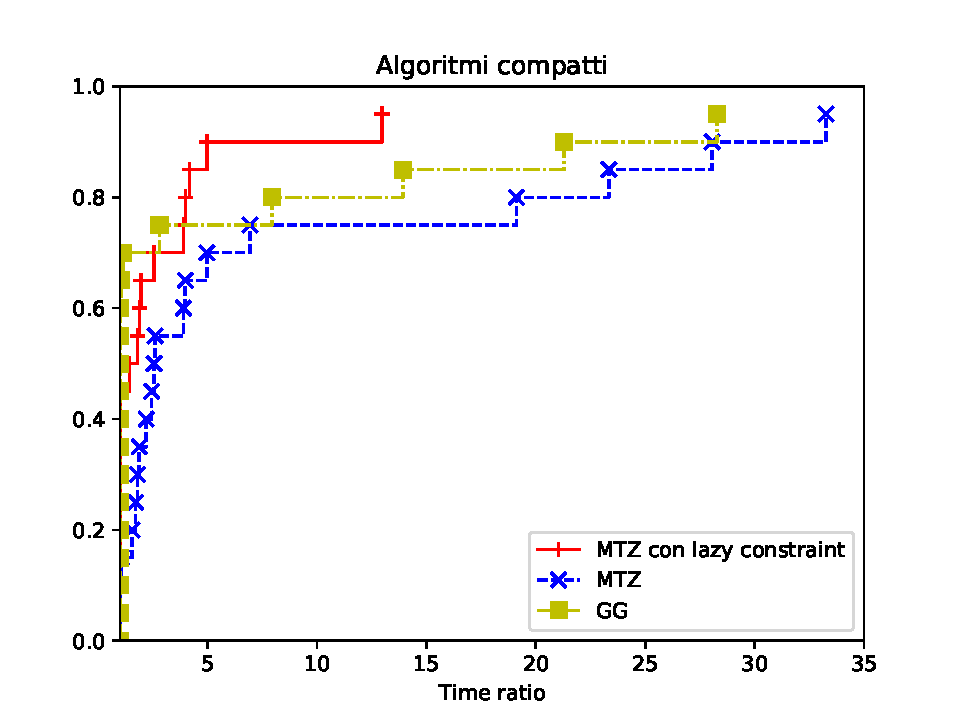
\includegraphics[scale=0.7]{Images/pp_compact}\\ 
  \caption{\footnotesize{Performance profile degli algoritmi compatti.}}
  \label{pp_compact} 
\end{center} 
\end{figure}
Gli algoritmi esatti, che non prevedono l'uso di modelli compatti, sono invece stati testati con un time limit di 10 minuti sul seguente dataset:
\begin{center}
\begin{multicols}{4}
\begin{itemize}
\item{a280.tsp}
\item{ali535.tsp}
\item{att48.tsp}
\item{att532.tsp}
\item{berlin52.tsp}
\item{bier127.tsp}
\item{burma14.tsp}
\item{ch130.tsp}
\item{ch150.tsp}
\item{d198.tsp}
\item{d493.tsp}
\item{d657.tsp}
\item{eil51.tsp}
\item{eil76.tsp}
\item{eil101.tsp}
\item{fl417.tsp}
\item{gil262.tsp}
\item{gr96.tsp}
\item{gr137.tsp}
\item{gr202.tsp}
\item{gr229.tsp}
\item{gr431.tsp}
\item{gr666.tsp}
\item{kroA100.tsp}
\item{kroA150.tsp}
\item{kroA200.tsp}
\item{kroB100.tsp}
\item{kroB150.tsp}
\item{kroB200.tsp}
\item{kroC100.tsp}
\item{kroD100.tsp}
\item{kroE100.tsp}
\item{lin105.tsp}
\item{lin318.tsp}
\item{p654.tsp}
\item{pcb442.tsp}
\item{pr76.tsp}
\item{pr107.tsp}
\item{pr124.tsp}
\item{pr136.tsp}
\item{pr144.tsp}
\item{pr152.tsp}
\item{pr226.tsp}
\item{pr299.tsp}
\item{pr439.tsp}
\item{rat99.tsp}
\item{rat195.tsp}
\item{rat575.tsp}
\item{rat783.tsp}
\item{rd100.tsp}
\item{rd400.tsp}
\item{st70.tsp}
\end{itemize}
\end{multicols}
\end{center}
Dall'analisi dei risultati ottenuti (Figura \ref{pp_exact}), è evidente come l'utilizzo del Branch \& Cut permetta di ottenere prestazioni migliori, ma soprattutto come l'utilizzo delle callback generiche abbia permesso di migliorare notevolmente le prestazioni, rispetto alla versione priva di esse.\\
L'utilizzo del patching ha avuto maggior effetto soprattutto nella prima parte dell'esecuzione del programma, in cui risulta essere molto di aiuto per CPLEX nel raggiungere l'ottimo. Successivamente le soluzioni passate al risolutore MIP, mediante le heuristic callback, vengono scartate da quest'ultimo sempre più spesso.\\
\begin{figure}[H] 
\begin{center} 
  % Requires \usepackage{graphicx} 
  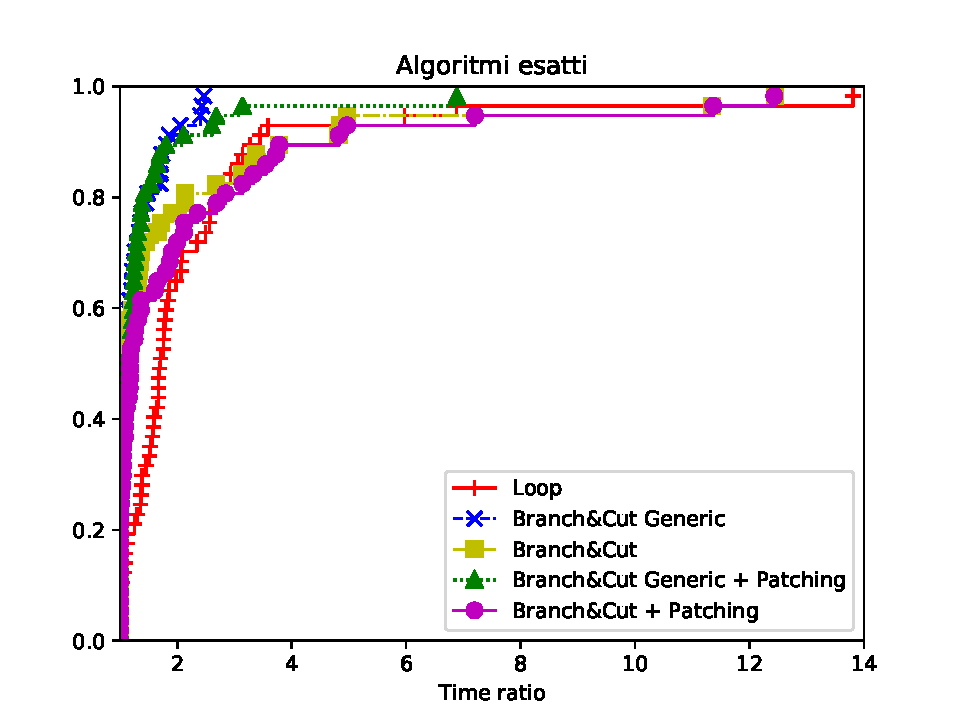
\includegraphics[scale=0.75]{Images/pp_exact}\\ 
  \caption{\footnotesize{Performance profile dei tempi di esecuzione degli algoritmi esatti implementati.}}
  \label{pp_exact} 
\end{center} 
\end{figure}
In Figura \ref{pp_random_seed} viene confrontato invece l'algoritmo loop attraverso l'utilizzo di diversi seed, ponendo l'attenzione su come la performance variability influenzi le prestazioni delle varie soluzioni implementative.
Il performance profile riportato in Figura \ref{pp_gap} confronta i risultati ottenuti mediante l'utilizzo dell'algoritmo loop nella sua versione classica con quelli ottenuti applicando la sua versione euristica. Nel grafico realizzato, le varianti euristiche individuano inizialmente una soluzione utilizzando il gap relativo evidenziato 
nel grafico ed in seguito impostano nuovamente il gap al valore di default ed individuano la soluzione ottima.
\begin{figure}[H] 
\begin{center} 
  % Requires \usepackage{graphicx} 
  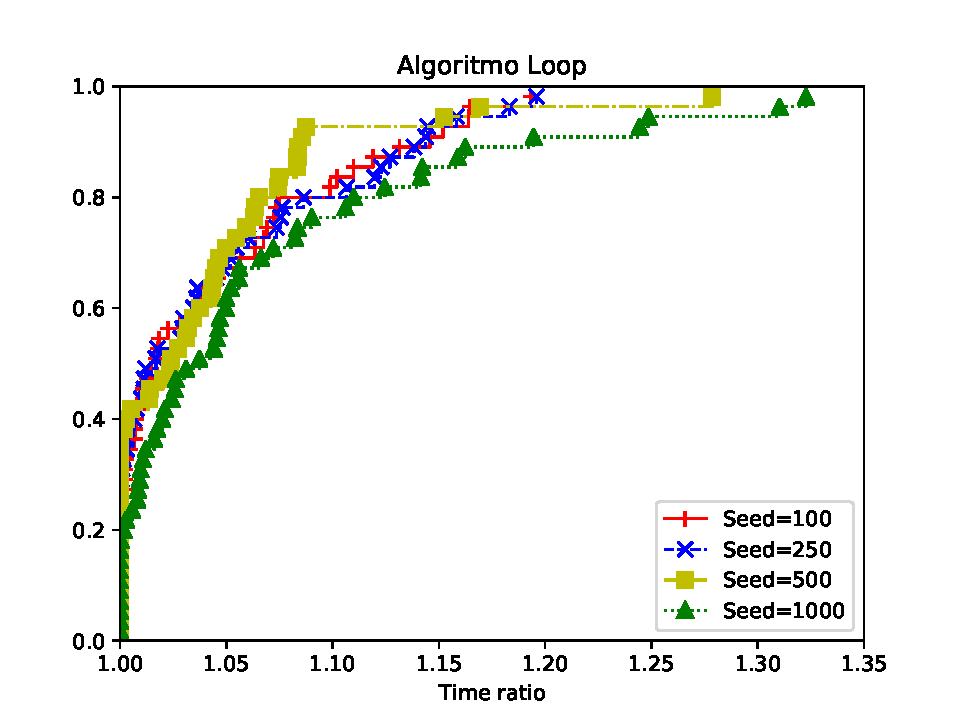
\includegraphics[scale=0.7]{Images/pp_random_seed}\\ 
  \caption{\footnotesize{Performance profile dei tempi di esecuzione dell'algoritmo loop al variare del seed.}}
  \label{pp_random_seed} 
\end{center} 
\end{figure}
\begin{figure}[H] 
\begin{center} 
  % Requires \usepackage{graphicx} 
  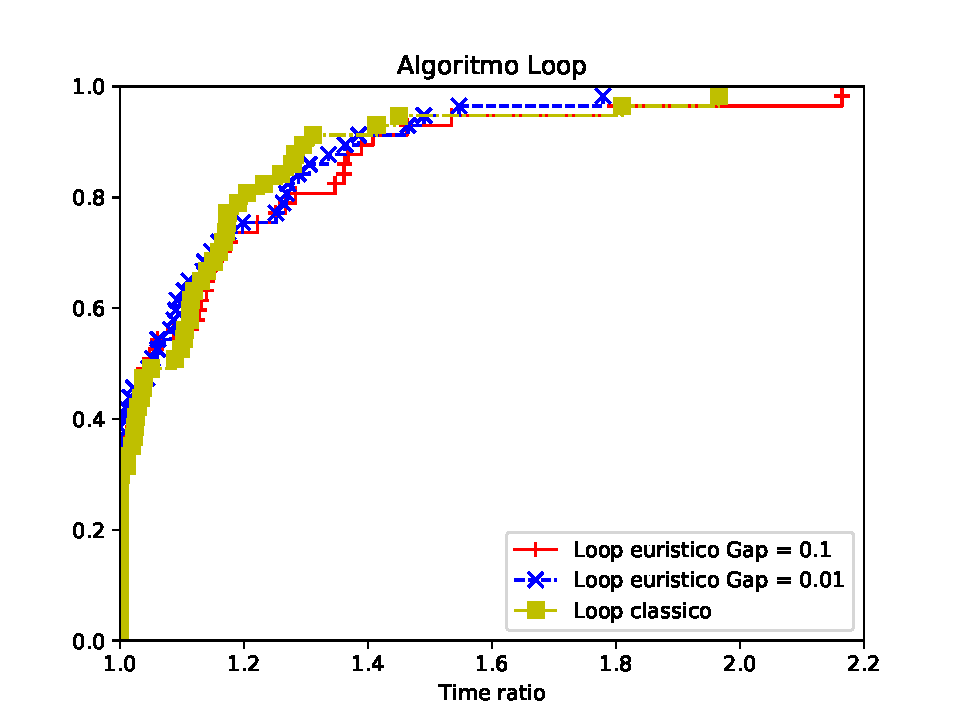
\includegraphics[scale=0.7]{Images/pp_gap}\\ 
  \caption{\footnotesize{Performance profile dei tempi di esecuzione dell'algoritmo loop euristico al variare del gap.}}
  \label{pp_gap} 
\end{center} 
\end{figure}

\vspace{2cm}
\subsection{Algoritmi math-euristici}
Gli algoritmi math-euristici sviluppati sono stati testati sul seguente insieme di istanze, con un time limit 10 minuti:
\begin{center}
\begin{multicols}{3}
\begin{itemize}
\item{a280.tsp}  
\item{att532.tsp} 
\item{bier127.tsp}
\item{d198.tsp}   
\item{d493.tsp}   
\item{eil76.tsp}  
\item{eil101.tsp} 
\item{fl417.tsp}  
\item{gr137.tsp}  
\item{gr202.tsp}  
\item{lin105.tsp} 
\item{lin318.tsp} 
\item{pcb442.tsp} 
\item{pr144.tsp}  
\item{pr264.tsp}  
\item{pr299.tsp}  
\item{pr439.tsp}  
\item{rat575.tsp} 
\item{rd400.tsp}  
\item{u159.tsp}
\end{itemize}
\end{multicols}
\end{center}
Analizzando i risultati ottenuti in Figura \ref{pp_math-heuristic} e \ref{pp_math-heuristic_zoom}) risulta evidente come le prestazioni dell'algoritmo Hard fixing siano migliori, sia nella variante che utilizza le callback generiche che in quella che non ne fa uso, rispetto ad entrambe le soluzioni ottenute dal Soft fixing.
\begin{figure}[h] 
\begin{center} 
  % Requires \usepackage{graphicx} 
  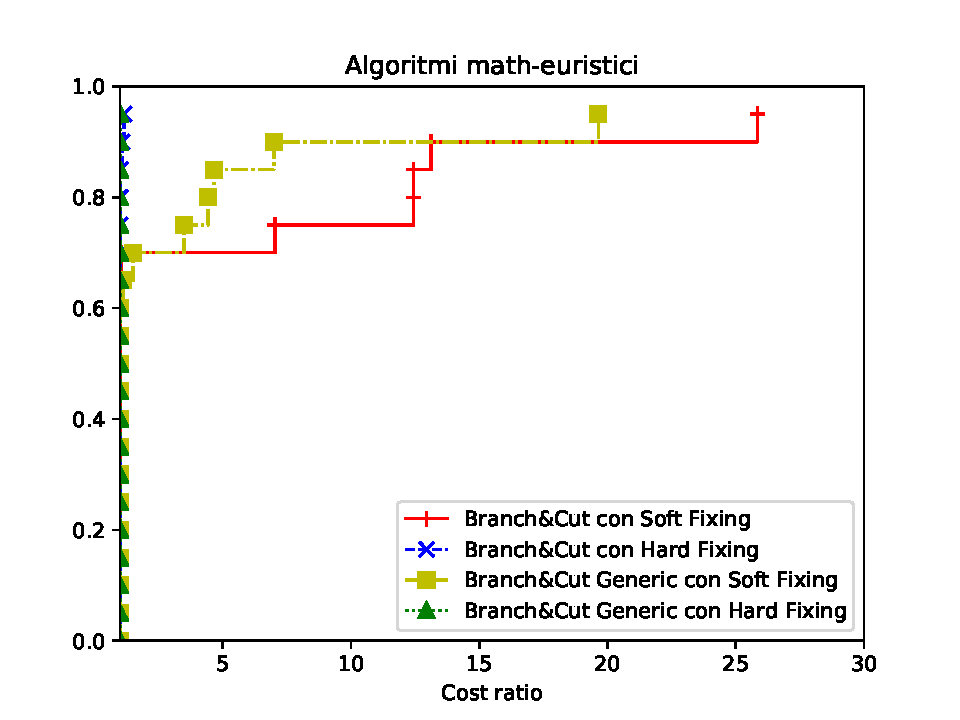
\includegraphics[scale=0.8]{Images/pp_math-heuristic}\\ 
  \caption{\footnotesize{Confronto degli algoritmi math-euristici in base al costo della soluzione ottenuta.}}
  \label{pp_math-heuristic} 
\end{center} 
\end{figure}

\begin{figure}[h] 
\begin{center} 
  % Requires \usepackage{graphicx} 
  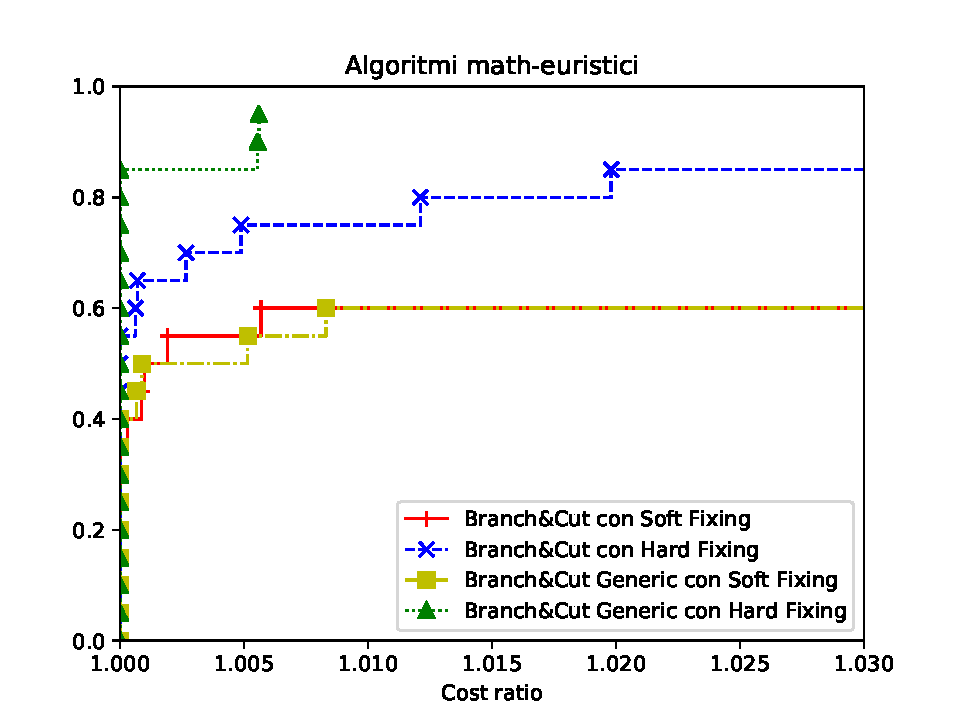
\includegraphics[scale=0.8]{Images/pp_math-heuristic_zoom}\\ 
  \caption{\footnotesize{Dettaglio del confronto degli algoritmi math-euristici in base al costo della soluzione ottenuta.}}
  \label{pp_math-heuristic_zoom} 
\end{center} 
\end{figure}
\vspace{10cm}
\subsection{Algoritmi euristici}
\subsubsection{Multi-start}\label{construction_perf}
In questa prima sezione, vengono analizzati i diversi algoritmi di costruzione implementati, applicando l'algoritmo multistart sulle seguenti istanze:
\begin{center}
\begin{multicols}{4}
\begin{itemize}
\item{a280.tsp}
\item{ali535.tsp}
\item{att532.tsp}
\item{d1291.tsp}
\item{d1665.tsp}
\item{d2103.tsp}
\item{d493.tsp}
\item{d657.tsp}
\item{dsj1000.tsp}
\item{fl1400.tsp}
\item{fl1577.tsp}
\item{fl417.tsp}
\item{gil262.tsp}
\item{gr431.tsp}
\item{gr666.tsp}
\item{lin318.tsp}
\item{nrw1379.tsp}
\item{p654.tsp}
\item{pcb1173.tsp}
\item{pcb442.tsp}
\item{pr1002.tsp}
\item{pr299.tsp}
\item{pr439.tsp}
\item{rat575.tsp}
\item{rat783.tsp}
\item{rd400.tsp}
\item{rl1304.tsp}
\item{rl1323.tsp}
\item{rl1889.tsp}
\item{u1060.tsp}
\item{u1432.tsp}
\item{u1817.tsp}
\item{u574.tsp}
\item{u724.tsp}
\item{vm1084.tsp}
\item{vm1748.tsp}
\end{itemize}
\end{multicols}
\end{center}

In Figura \ref{pp_construction}, viene riportato il performance profile ottenuto dall'esecuzione dell'algoritmo multistart, generando 40 differenti soluzioni per ciascuna istanza del problema e restituendo solo il costo della migliore tra queste.\\
Le soluzioni di costo minore sono quelle restituite dall'algoritmo Nearest Neighborhood, in particolare con l'aggiunta del metodo GRASP. 
Inoltre si è notato come il tempo necessario alla definizione di una soluzione mediante il metodo insertion sia molto elevato. 
\begin{figure}[h] 
\begin{center} 
  % Requires \usepackage{graphicx} 
  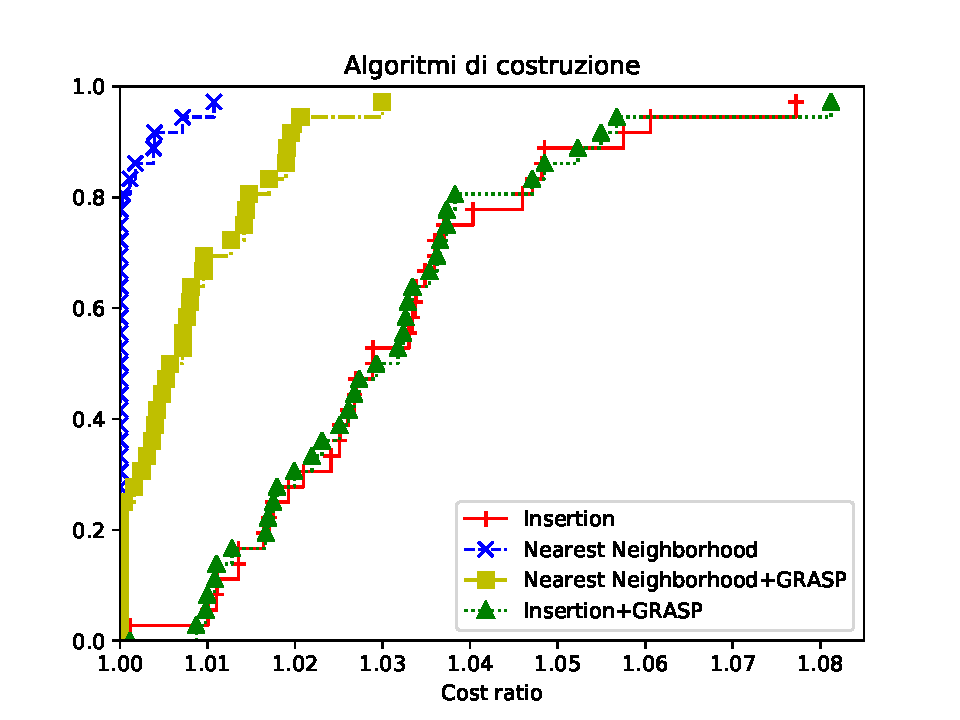
\includegraphics[scale=0.8]{Images/pp_construction}\\ 
  \caption{\footnotesize{Confronto dei vari multistart in base all'algoritmo di costruzione utilizzato.}}
  \label{pp_construction} 
\end{center} 
\end{figure}
\subsubsection{Algoritmi meta-euristici}
Tutti gli algoritmi meta-euristici sviluppati, escluso il genetico, prevedono la possibilità di utilizzare uno qualsiasi tra gli algoritmi di costruzione definiti, semplicemente associando specifici valori a delle macro.\\
Per i motivi descritti nella sezione precedente, gli algoritmi sono stati testati però utilizzando il metodo di costruzione Nearest Neighborhood e con un time limit di 10 minuti. In questi test, è stata impostata una macro che permette al multistart di essere eseguito in multithreading in questo intervallo di tempo, generando iterativamente 8 soluzioni alla volta. Il primo dataset su cui sono stati svolti i test è il seguente:
\begin{center}
\begin{multicols}{3}
\begin{itemize}
\item{d1291.tsp}
\item{d1655.tsp} 
\item{d2103.tsp} 
\item{dsj1000.tsp}
\item{fl1400.tsp} 
\item{fl1577.tsp} 
\item{nrw1379.tsp} 
\item{pcb1173.tsp} 
\item{pr1002.tsp}
\item{pr2392.tsp}
\item{rl1304.tsp}
\item{rl1323.tsp}
\item{rl1889.tsp}
\item{u1060.tsp} 
\item{u1432.tsp}
\item{u1817.tsp}
\item{u2152.tsp}
\item{u2319.tsp}
\item{vm1084.tsp}
\item{vm1748.tsp}
\end{itemize}
\end{multicols}
\end{center}
L'algoritmo genetico non è stato applicato a questo primo dataset. Il motivo di tale scelta, riguarda il tempo di calcolo troppo elevato per la generazione della popolazione.\\
Per tale motivo tutti gli algoritmi meta-euristici sono stati testati nuovamente sulle seguenti istanze di dimensione minore, per ottenere un confronto più equo della soluzione del genetico con le altre:
\begin{center}
\begin{multicols}{3}
\begin{itemize}
\item{a280.tsp}
\item{bier127.tsp}
\item{ch130.tsp}
\item{ch150.tsp}
\item{d198.tsp}
\item{gil262.tsp}
\item{gr137.tsp}
\item{kroA150.tsp}
\item{kroA200.tsp}
\item{kroB150.tsp}
\item{kroB200.tsp}
\item{pr124.tsp}
\item{pr136.tsp}
\item{pr144.tsp}
\item{pr152.tsp}
\item{pr226.tsp}
\item{pr264.tsp}
\item{pr299.tsp}
\item{rd400.tsp}
\item{u159.tsp}
\end{itemize}
\end{multicols}
\end{center}
Analizzando i risultati ottenuti in entrambi i test (Figura \ref{pp_heuristic} e \ref{pp_genetic}), le soluzioni con costo minore sono quelle ottenute mediante il Simulated Annealing e il VNS ibribo. Nel primo caso, con istanze di grandezza maggiore, la seconda implementazione del VNS genera soluzioni di costo minore mentre nel confronto con l'algoritmo genetico, la prima implementazione del VNS risulta migliore.\\
I grafici in Figura \ref{cost_vns}, \ref{cost_tabu}, \ref{cost_sa} e \ref{cost_genetic} rappresentano invece l'andamento del costo applicando rispettivamente il VNS ibrido, il Tabu Search, il Simulated Annealing e l'algoritmo genetico all'istanza \textit{bier127.tsp}.
\begin{figure}[h] 
\begin{center} 
  % Requires \usepackage{graphicx} 
  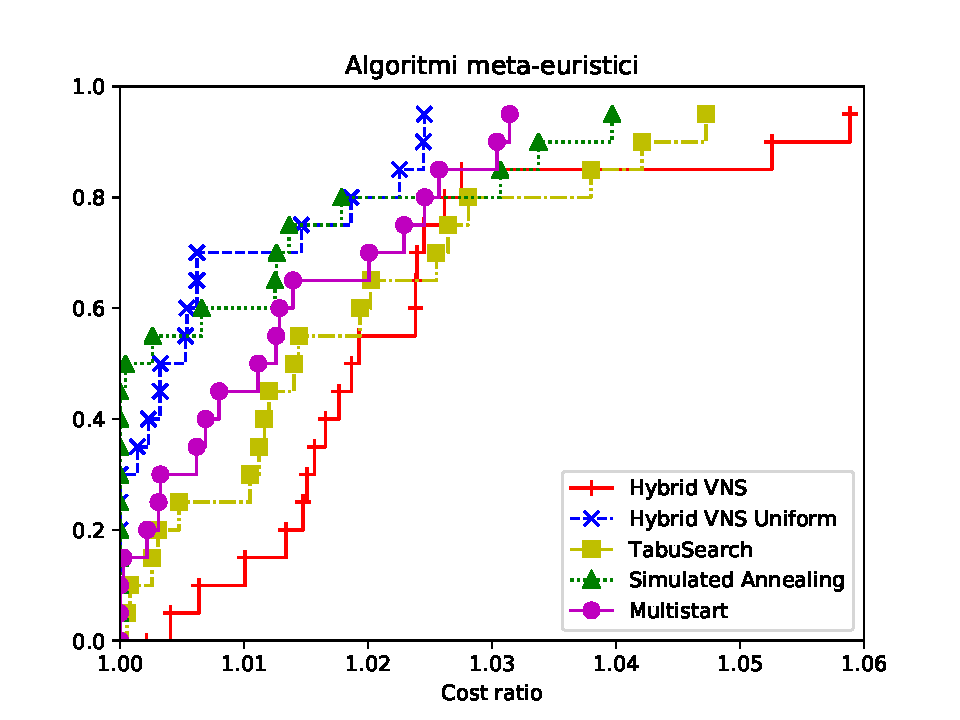
\includegraphics[scale=0.8]{Images/pp_heuristic}\\ 
  \caption{\footnotesize{Confronto dei costi delle soluzioni ottenute mediante gli algoritmi meta-euristici, escluso il genetico.}}
  \label{pp_heuristic} 
\end{center}
\end{figure}
\begin{figure}[h] 
\begin{center} 
  % Requires \usepackage{graphicx} 
  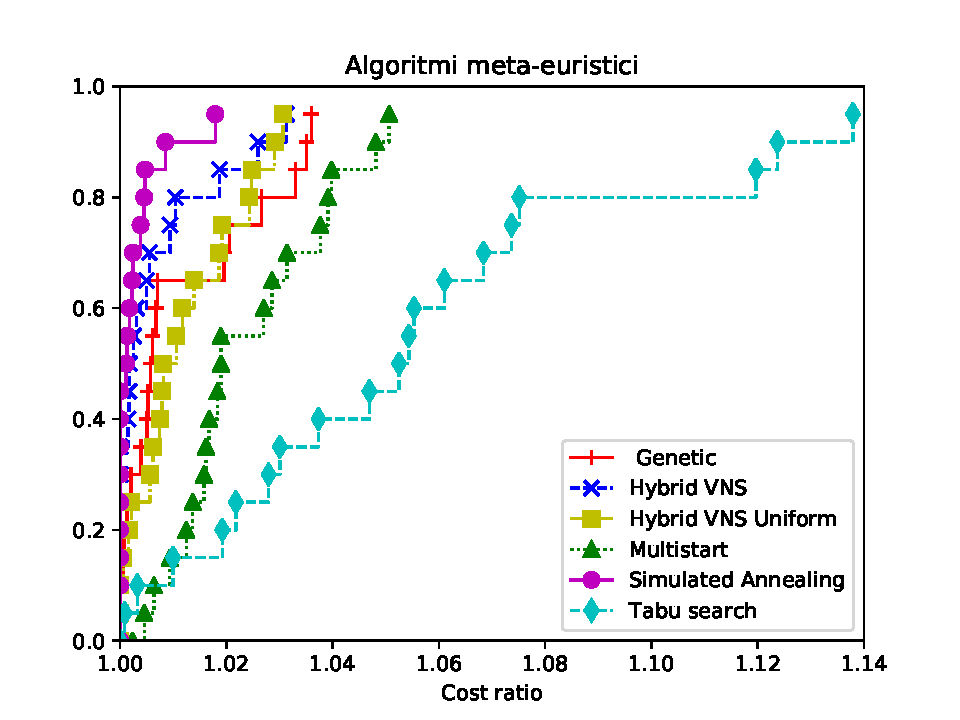
\includegraphics[scale=0.8]{Images/pp_genetic}\\ 
  \caption{\footnotesize{Confronto dei costi delle soluzioni ottenute mediante tutti gli algoritmi meta-euristici.}}
  \label{pp_genetic} 
\end{center} 
\end{figure}
\begin{figure}[h]
\begin{center} 
  % Requires \usepackage{graphicx} 
  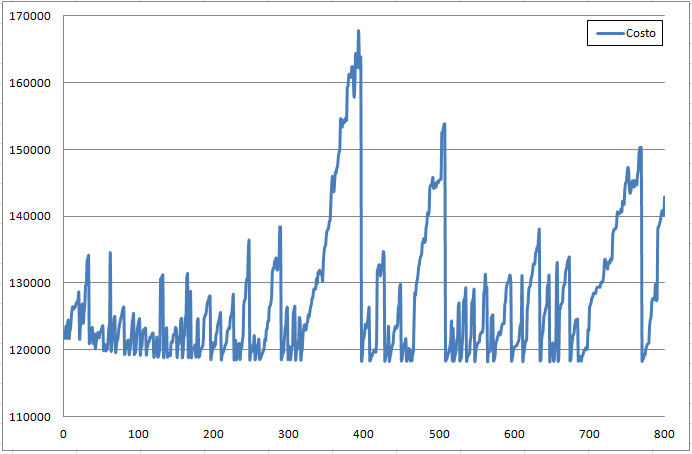
\includegraphics[scale=0.7]{Images/cost_vns}\\ 
  \caption{\footnotesize{Evoluzione del costo della soluzione attuale nell'algoritmo VNS.}}
  \label{cost_vns} 
\end{center} 
\end{figure}
\begin{figure}[h] 
\begin{center} 
  % Requires \usepackage{graphicx} 
  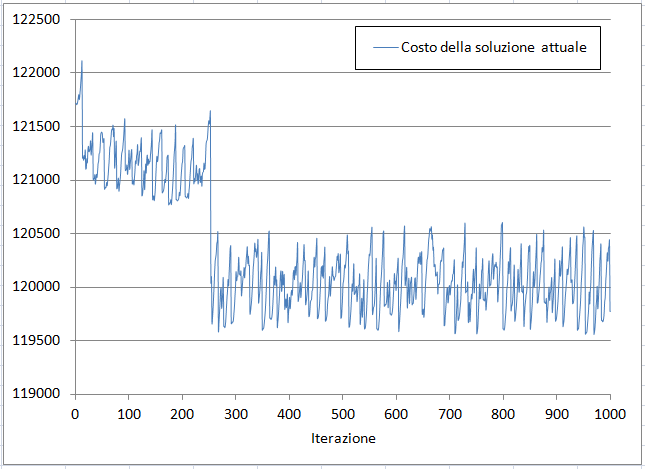
\includegraphics[scale=0.7]{Images/cost_tabu}\\ 
  \caption{\footnotesize{Evoluzione del costo della soluzione attuale nell'algoritmo Tabu search.}}
  \label{cost_tabu} 
\end{center} 
\end{figure}
\begin{figure}[h] 
\begin{center} 
  % Requires \usepackage{graphicx} 
  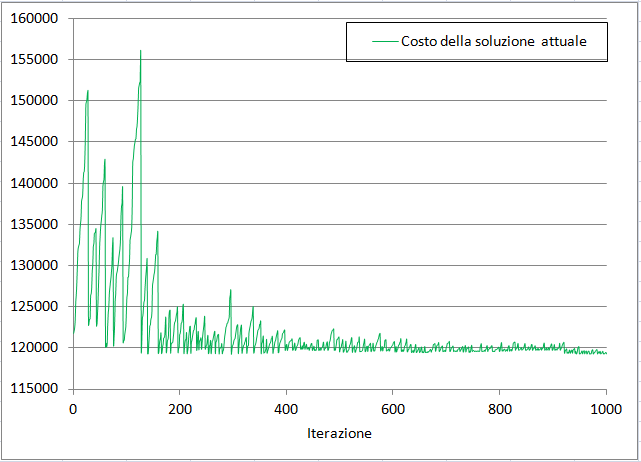
\includegraphics[scale=0.7]{Images/cost_sa}\\ 
  \caption{\footnotesize{Evoluzione del costo della soluzione attuale nell'algoritmo Simulated Annealing.}}
  \label{cost_sa} 
\end{center} 
\end{figure}
\begin{figure}[h]
\begin{center} 
  % Requires \usepackage{graphicx} 
  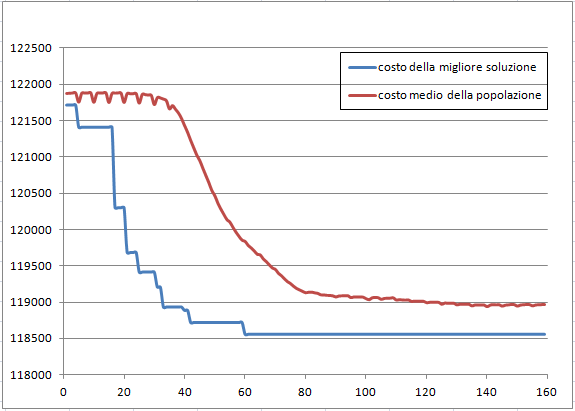
\includegraphics[scale=0.7]{Images/cost_genetic}\\ 
  \caption{\footnotesize{Evoluzione del costo medio della popolazione e del costo della soluzione migliore nell'algoritmo genetico.}}
  \label{cost_genetic} 
\end{center} 
\end{figure}
\chapter{Appendice}
In questa sezione verranno approfondite alcune funzioni di CPLEX necessarie ad implementare gli algoritmi descritti nei capitoli precedenti. Inoltre vengono analizzati tutti gli altri programmi, utilizzati nella stampa delle soluzioni e nell'analisi delle performance.

\section{CPLEX}
\subsection{Funzioni}
\subsubsection{Costruzione modello}
Per poter costruire il modello da analizzare, come prima cosa, è necessario creare un puntatore alle due strutture dati utilizzate da CPLEX.
\lstinputlisting[caption={\footnotesize{modelTSP.txt}}, style=code, firstnumber=1, firstline=27, lastline=29, label=tsp_model, language=c]{Source/modelTSP.txt}
La funzione alla riga 2 alloca la memoria necessaria e riempie la struttura con valori di default. Nel caso in cui non termini con successo memorizza un codice d'errore in \textit{\&error}.\\
La funziona invocata nella riga successiva, invece, associa la struttura LP all'ENV che gli viene fornito. Il terzo parametro passato, nell'esempio "TSP", sarà il nome del modello creato.
Al termine di queste operazioni verrà quindi creato un modello vuoto. All'interno del nostro programma per inizializzarlo è stata costruita la seguente funzione:
\begin{center}
\begin{tabular}{c}
\begin{lstlisting}[linewidth=320pt, basicstyle=\footnotesize\sffamily,] 
void cplex_build_model(istanza_problema, env , lv);
\end{lstlisting}
\end{tabular}
\end{center}
\begin{table}[h]
\centering
\begin{tabular}{rl}
\textbf{istanza\_problema: } & {puntatore alla struttura che contiene} \\
&  {l'istanza del problema (letta dal file TSPlib)} \\
\textbf{env: } & {puntatore di tipo CPXENVptr alla}\\
& {struttura ENV precedentemente creata}\\
\textbf{lp: } & {puntatore di tipo CPXLPptr alla}\\
& {struttura LP  precedentemente creata}\\
\end{tabular}
\end{table}
All'interno di \textbf{cplex\_build\_model()} viene aggiunta una colonna alla volta al modello, definendo quindi anche la funzione obiettivo. Le variabili aggiunte corrispondono agli archi del grafo e per ciascuno di questi viene calcolato il costo come distanza euclidea. La funzione necessaria ad inserire colonne e definire la funzione di costo è la seguente:
\vspace{0.5cm}
\begin{center}
\begin{tabular}{c}
\begin{lstlisting}[linewidth=350pt, basicstyle=\footnotesize\sffamily,]     
CPXnewcols(env, lp, num_colonne, costi, lower_bound, 
           upper_bound, tipi_variabili, nomi_variabili);
\end{lstlisting}
\end{tabular}
\end{center}
\begin{table}[h]
\begin{tabular}{rl}
\textbf{env:} & {puntatore di tipo CPXENVptr alla}\\
& {struttura ENV precedentemente creata} \\
\textbf{lp:} & {di tipo CPXLPptr, è un puntatore alla struttura LP}\\
& {precedentemente creata}\\
\textbf{num\_colonne:} & {numero di colonne da inserire} \\    
\textbf{costi:} & {vettore dei costi relativi agli archi da inserire} \\
\textbf{lower\_bound:} & {vettore contenente i lower bound dei valori}\\
& {assumibili dalle variabili da inserire}\\              
\textbf{upper\_bound:} & {vettore contenente gli upper bound dei valori}\\
&  {assumibili dalle variabili da inserire} \\
\textbf{tipi\_variabili:} & {vettore contenente la tipologia delle variabili}\\
& da inserire\\
\textbf{nomi\_variabili:} & {vettore di stringhe contenenti i nomi}\\
& {delle variabili da inserire}
\end{tabular}
\end{table}
La generica colonna \textbf{i}, aggiunta dalla funzione, sarà definita dalle informazioni contenute all'interno della posizione \textbf{i} degli array, ricevuti come parametri. Nel programma elaborato durante il corso, viene aggiunta una colonna alla volta all'interno del modello. Per far ciò, è necessario comunque utilizzare riferimenti alle informazioni da inserire, in modo da ovviare il problema riguardante la tipologia di argomenti richiesti, che sono array. Ad esempio, nel nostro caso, la tipologia di una nuova variabile inserita sarà un riferimento al carattere \textbf{'B'}, che la identifica come binaria.\\
Per poter inserire il primo insieme di vincoli del problema\\
$$
\underset{e\in \delta(v)}\sum{\;x_e} = 2\;\;\;\;\;\;\;\;\;\;\;\;\;\;\;\;\;\;\forall\;v\in V \\\\
$$
\\
viene invece sfruttata la seguente funzione:
\begin{center}
\begin{tabular}{c}
\begin{lstlisting}[linewidth=330pt, basicstyle=\footnotesize\sffamily,]     
 CPXnewrows(env, lp, numero_righe,termini_noti,
            tipi_vincoli, range_valori, nomi_vincoli);
\end{lstlisting}
\end{tabular}
\end{center}
\begin{table}[h]
\begin{tabular}{rl}
\textbf{env:} & {puntatore di tipo CPXENVptr alla struttura ENV}\\
& {precedentemente creata}\\
\textbf{lp:} & {puntatore di tipo CPXLPptr alla struttura LP}\\
& {precedentemente creata}\\
\textbf{numero\_righe:} & {numero di righe (vincoli) da inserire}\\
\textbf{termini\_noti:} & {vettore dei termini noti dei vincoli}\\
\textbf{tipi\_vincoli:} & {vettore di caratteri che specifica il tipo di vincoli}\\
&{da inserire. Ogni carattere può assumere:}\\
&{\textit{'L'} per vincolo $\leq$}\\
&{\textit{'E'} per vincolo $=$}\\
&{\textit{'G'} per vincolo $\geq$}\\
&{\textit{'R'} per vincolo definito in un intervallo}\\
\textbf{range\_valori:} & {vettore di range per i valori di ogni vincolo}\\
& {(nel nostro caso è NULL)} \\
\textbf{nomi\_vincoli} & vettore di stringhe contenenti i nomi  \\
                  & delle variabili da inserire
\end{tabular}
\end{table}
In modo analogo all'inserimento delle colonne, nel nostro programma viene aggiunta una riga alla volta nel modello. L'\textbf{i}-esima riga aggiunta corrisponderà al vincolo imposto sul nodo \textbf{i}-esimo, imponendo a 1 il coefficiente della variabile $x_{k,j}$ se $k=i$ $j=i$ per ogni variabile del modello.\\\\
\subsubsection{Lazy constraints}
Nel caso in cui si voglia sfruttare la possibilità di verificare se è stato rispettato un vincolo, solo al termine della computazione della soluzione, è necessario inserire un "lazy constraint". Per fare ciò viene utilizzata la seguente funzione:
\begin{center}
\begin{tabular}{c}
\begin{lstlisting}[linewidth=380pt, basicstyle=\footnotesize\sffamily,]     
CPXaddlazyconstraints(env, lp, num_vincoli, nnz, 
					termine_costante, tipo_vincolo, posizione_iniziale,
					indici, valori, nome_vincolo);
\end{lstlisting}
\end{tabular}
\end{center}
\begin{table}[h]
\begin{tabular}{rl}
\textbf{env:} & {puntatore di tipo CPXENVptr alla struttura ENV}\\
& {precedentemente creata}\\
\textbf{lp:} & {puntatore di tipo CPXLPptr alla struttura LP}\\
& {precedentemente creata}\\
\textbf{num\_vincoli:} & {numero di vincoli da inserire}\\
\textbf{nnz:} & {vettore con il numeri di variabili per ogni vincolo}\\ 
\textbf{termine\_costante:} & {vettore dei termini noti dei vincoli}\\
\textbf{tipi\_vincoli:} & {vettore di caratteri che specifica il tipo di vincoli}\\
&{da inserire. Ogni carattere può assumere:}\\
&{\textit{'L'} per vincolo $\leq$}\\
&{\textit{'E'} per vincolo $=$}\\
&{\textit{'G'} per vincolo $\geq$}\\
&{\textit{'R'} per vincolo definito in un intervallo}\\
\textbf{posizione\_iniziale:} & {vettore con le posizione iniziali dei coefficienti nei vincoli}\\
\textbf{indici:} & {vettore di vettori contenenti gli indici delle variabili }\\
& {appartenenti al vincolo}\\
\textbf{valori:} & {vettore di vettori con i coefficienti delle variabili del vincolo}\\
\textbf{nome\_vincolo:} & {vettore con i nomi dei vincoli}\\
\end{tabular}
\end{table}
In modo analogo alle due funzioni precedentemente descritte per l'aggiunta di righe e colonne, nel nostro modello viene inserito un vincolo per volta. Per impostare correttamente i coefficienti delle variabili presenti nel vincolo, vengono sfruttati i due array \textit{indici} e \textit{valori}. Come rappresentato in Figura \ref{lazy_constraints}, all'interno della posizione \textit{i}-esima del vettore di indici è presente la posizione dell'\textit{i}-esima variabile del vincolo da inserire (nell'esempio in figura $indici[i]=j$). Mentre l'\textit{i}-esima posizione del vettore di valori contiene il corrispondente  coefficiente (in questo caso $c_j$).
\begin{figure}[h] 
\begin{center} 
  % Requires \usepackage{graphicx} 
  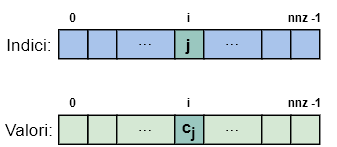
\includegraphics[scale=0.5]{Images/lazy_constraints}\\ 
  \caption{\footnotesize{Array lazy constraints}}
  \label{lazy_constraints} 
\end{center} 
\end{figure}
\subsubsection{Calcolo della soluzione}
Per ottenere la soluzione ottima del problema di ottimizzazione del problema correlato al modello definito in cplex, vengono utilizzate due fasi:
\begin{itemize}
\item{\textbf{Risoluzione del problema di ottimizzazione}\\
\begin{center}
\begin{tabular}{c}
\begin{lstlisting}[linewidth=120pt, basicstyle=\footnotesize\sffamily,]
CPXmipopt(env, lp);
\end{lstlisting}
\end{tabular}
\end{center}
\begin{table}[h]
\centering
\begin{tabular}{rl}
\textbf{env:} & {puntatore di tipo CPXENVptr alla struttura ENV}\\
& {precedentemente creata}\\
\textbf{lp:} & {puntatore di tipo CPXLPptr alla struttura LP}\\
& {precedentemente creata}\\
\end{tabular}
\end{table}
}
\item{\textbf{Ottenimento della soluzione}\\
\begin{center}
\begin{tabular}{c}
\begin{lstlisting}[linewidth=230pt, basicstyle=\footnotesize\sffamily,]
CPXgetx(env, lp, x, inizio, fine);
\end{lstlisting}
\end{tabular}
\end{center}
\begin{table}[h]
\centering
\begin{tabular}{rl}
\textbf{env:} & {puntatore di tipo CPXENVptr alla struttura ENV}\\
& {precedentemente creata}\\
\textbf{lp:} & {puntatore di tipo CPXLPptr alla struttura LP}\\
& {precedentemente creata}\\
\textbf{x:} & {puntatore a un vettore di double in cui verranno salvati}\\
\end{tabular}
\end{table}
\begin{table}[h]
\centering
\begin{tabular}{rl}
& {i valori delle variabili ottenuti dalla soluzione ottima}\\
\textbf{inizio:} & {primo indice della variabile di cui si vuole memorizzare}\\
& {ed analizzare il valore}\\
\textbf{fine:} & {indice dell'ultima variabile di cui si vuole memorizzare}\\
& {ed analizzare il valore}\\
\end{tabular}
\end{table}
Questa funzione salva in x tutte le variabili che hanno indice $i\in [inizio, fine]$ e quindi x deve essere un vettore di almeno $fine-inizio+1$ valori. Nel nostro programma, vengono analizzati i valori di tutte le variabili in gioco.\\
Per questo motivo \textbf{inizio=0} e \textbf{fine=num\_colonne - 1}\footnote{numero di variabili=CPXgetnumcols(env,lp);}\footnote{numero di vincoli=CPXgetnumrows(env,lp);}. In seguito il nostro programma analizza la correttezza della soluzione svolgendo la verifica su:
\begin{itemize}
\item{\textit{valori assunti dalle variabili}\\
ciascun $x_{i,j}$ assume valore $0$ o $1$ con una tolleranza di $\epsilon=10^{-5}$}
\item{\textit{grado di ciascun nodo}\\
il tour è composto al massimo da due archi che toccano lo stesso nodo}
\end{itemize}
}
\end{itemize}
\subsection{Parametri}\label{param}
Con le seguenti funzioni è possibile modificare i parametri di impostazione di CPLEX, altrimenti impostati ai valori di default.
Nel caso in cui si tratti di parametri di tipo INT è necessario invocare:\\
\begin{center}
\begin{tabular}{c}
\begin{lstlisting}[linewidth=330pt, basicstyle=\footnotesize\sffamily,]     
CPXsetintparam(env, numero_parametro, nuovo_valore);
\end{lstlisting}
\end{tabular}
\end{center}
mentre se di tipo DOUBLE:\\
\begin{center}
\begin{tabular}{c}
\begin{lstlisting}[linewidth=330pt, basicstyle=\footnotesize\sffamily,]     
CPXsetdblparam(env, numero_parametro, nuovo_valore);
\end{lstlisting}
\end{tabular}
\end{center}
In entrambe le funzioni
\begin{table}[h]
\begin{tabular}{rl}
\textbf{env:} & {puntatore di tipo CPXENVptr alla struttura ENV}\\
& {di cui si vogliono cambiare i parametri}\\
\textbf{numero\_parametro:} & {intero corrispondente al parametro da modificare (vedi Tabella \ref{param_table})}\\
\textbf{nuovo\_valore:} & {nuovo valore (rispettivamente intero o double)}\\
& {del parametro}\\
\end{tabular}
\end{table}

\begin{table}[h]
\centering
\begin{tabular}{|l|l|}
\hline
{\textbf{CPX\_PARAM\_EPGAP}} & {tolleranza dell'intervalo tra la migliore funzione obiettivo intera e la funzione obiettivo del miglior nodo rimanente.}\\
{\textbf{CPX\_PARAM\_NODELIM}} & {massimo numero di nodi da risolvere prima che l'algoritmo termini senza aver aggiunto l'ottimalità (0 impone di fermarsi alla radice).}\\
{\textbf{CPX\_PARAM\_POPULATELIM}} & {Limita il numero di soluzioni MIP generate per il pool di soluzioni durante ogni chiamata alla procedura populate.}\\
{\textbf{CPX\_PARAM\_SCRIND}} & {visione o meno dei messaggi di log di CPLEX}\\
\hline
\end{tabular}
\end{table}
\subsection{Costanti utili}
Di seguito sono riportate alcune macro utili di CPLEX, insieme ai loro corrispondenti valori:
\begin{table}[h]
\begin{tabular}{|r|l|}
\hline
\textbf{CPX\_ON} & {\textbf{1}}\\
{} & {valore da assegnare ad alcuni parametri per abilitarli}\\
\hline
\textbf{CPX\_OFF} & {0}\\
{} & {valore da assegnare ad alcuni parametri per disabilitarli}\\
\hline
\textbf{CPX\_INFBOUND} & {$+\infty$}\\
{} & {massimo valore intero utilizzabile in CPLEX}\\
\hline
\end{tabular}
\end{table}

\section{Gnuplot}\label{gnuplot}
Una volta ottenuta la soluzione del problema di ottimizzazione, viene disegnato il grafo per facilitare all'utente la comprensione della sua correttezza. Per fare ciò viene utilizzato Gnuplot, un programma di tipo command-driven.\\
Per poterlo utilizzare all'interno del proprio programma esistono due metodi:
\begin{itemize}
\item{Collegare la libreria ed invocare le sue funzioni all'interno del nostro programma}
\item{Collegare l'eseguibile interattivo al proprio programma. In questo caso i comandi deve essere passati all'eseguibile attraverso un file di testo e l'utilizzo di un pipe.}\\
\end{itemize}
In questa trattazione è stato scelto il secondo metodo. All'interno del file è possibile specificare a Gnuplot le caratteristiche grafiche che deve aver il grafo. Di seguito viene riportato un esempio di tale file.\\

\lstinputlisting[caption={\footnotesize{style.txt}}, style=code, firstnumber=1, firstline=1, lastline=12, label=style_example]{Source/style_example.txt}

Nell'esempio sopra riportato, nella prima parte viene definito lo stile, il colore delle linee e la tipologia di punti, che verrano in seguito visualizzati all'interno del grafico prodotto.\\In seguito viene effettuato il plot del grafo in una finestra, utilizzando il primo e secondo valore di ciascuna riga del file \textbf{solution.dat} come coordinate mentre il terzo valore viene utilizzato come etichetta.\\\\
Il file \textbf{solution.dat} contiene le informazioni relative alla soluzione del grafico in cui ciascuna riga ha la seguente forma:
\begin{lstlisting}[linewidth=290pt,basicstyle=\footnotesize\sffamily,]     
coordinata_x   coordinata_y   posizione_in_tour
\end{lstlisting}
\textbf{coordinata\_x} rappresenta la coordinata x del nodo;\\
\textbf{posizione\_in\_tour} rappresenta la coordinata y del nodo;\\
\textbf{posizione\_in\_tour} rappresenta l'ordine del nodo all'interno del tour, assunto come nodo di origine il nodo 1.\\\\
Il grafico viene generato dal comando \textbf{plot}, leggendo tutte le righe non vuote e disegnando un punto nella posizione \textbf{(coordinata\_x,coordinata\_y)} del grafico 2D. In seguito viene tracciata una linea solo tra coppie di punti, legati a righe consecutive non vuote all'interno di \textbf{solution.dat}.\\\\
Attraverso le istruzioni riportate nelle righe 10-12 di \textbf{style.txt}, viene invece salvato il grafico appena generato nell'immagine \textbf{solution.png}.\\\\
Di seguito vengono riportate le varie fasi necessarie alla definizione di un pipe e al passaggio di questo al programma GNUplot:
\begin{itemize}
\item{\textbf{Definizione del pipe}
\lstinputlisting[style=code, firstnumber=1, firstline=1, lastline=1, label=style_example language=C]{Source/gnuplotC.txt}
dove \textbf{GNUPLOT\_EXE} è una stringa composta dal percorso completo dell'eseguibile di GNUplot, seguita dall'argomento \textbf{-persistent} (es. \textit{"D:/Programs/GNUplot/bin/gnuplot -persistent"}).
}
\item{\textbf{Passaggio delle istruzioni a GNUplot}
\lstinputlisting[style=code, firstnumber=2, firstline=2, lastline=10, label=style_example, language=C]{Source/gnuplotC.txt}
viene passata una riga alla volta, del file \textbf{style.txt}, a GNUplot mediante il pipe precedentemente creato.
}
\item{\textbf{Chiusura del pipe}
\lstinputlisting[style=code, firstnumber=11, firstline=11, lastline=11, label=style_example, language=C]{Source/gnuplotC.txt}
}
\end{itemize}

\section{perprof.py}
Il programma utilizzato per la creazione del performance profile dei diversi algoritmo è perprof.py\cite{salvagnin_perf}. Di seuito vengono riportati i principali argomenti da linea di comando che possono essere utilizzati:

\begin{table}[h]
\begin{tabular}{|r|l|}
\hline
\textbf{-D delimiter} & {spefica che delimiter verrà usato come separatore tra le parole in una riga}\\
\hline
\textbf{-M value} & {imposta value come il massimo valore di ratio (asse x)}\\
\hline
\textbf{-S value} & {value rappresenta la quantità che viene sommata a ciascun tempo di esecuzione prima di confrontarli. Utile per non enfatizzare di troppo differenze di pochi ms.}\\
\hline
\textbf{-L} & {stampa in scala logaritmica}\\
\hline
\textbf{-T value} & {nel file passato al programma, il TIME LIMIT=value}\\
\hline
\textbf{-P "title"} & {title è il titolo del plot}\\
\hline
\textbf{-X value} & {nome dell'asse x (default='Time Ratio')}\\
\hline
\textbf{-B} & {plot in bianco e nero}\\
\hline
\end{tabular}
\end{table}
Di seguito viene riportato un esempio dell'esecuzione del programma, del suo input e del suo output:
\begin{itemize}
\item{\textbf{comando}
\begin{center}
\begin{tabular}{c}
\begin{lstlisting}[linewidth=320pt, basicstyle=\footnotesize\sffamily,] 
python perfprof.py -D , -T 3600 -S 2 -M 20 esempio.csv pp.pdf -P "all instances, shift 2 sec.s"
\end{lstlisting}
\end{tabular}
\end{center}
}
\item{\textbf{file di input con i dati}\\
Viene riportato parte del contenuto di esempio.csv .
\begin{center}
\begin{tabular}{c}
\begin{lstlisting}[linewidth=320pt, basicstyle=\footnotesize\sffamily,] 
3, Alg1, Alg2, Alg3
model_1.lp, 2.696693, 3.272468, 2.434147
model_2.lp, 0.407689, 1.631921, 1.198957
model_3.lp, 0.333669, 0.432553, 0.966638
\end{lstlisting}
\end{tabular}
\end{center}
La prima riga deve necessariamente contenere in ordine il numero di algoritmi analizzati e i loro nomi. Nelle righe seguenti viene riportato invece il nome del file lp e i tempi di esecuzione elencati secondo la sequenza elencata nella prima riga.
Ogni campo di ciascuna riga deve essere separato dal delimitatore specificato all'avvio del programma attraverso l'opzione -D.
}
\item{\textbf{immagine di output}
\begin{figure}[h] 
\begin{center} 
  % Requires \usepackage{graphicx} 
  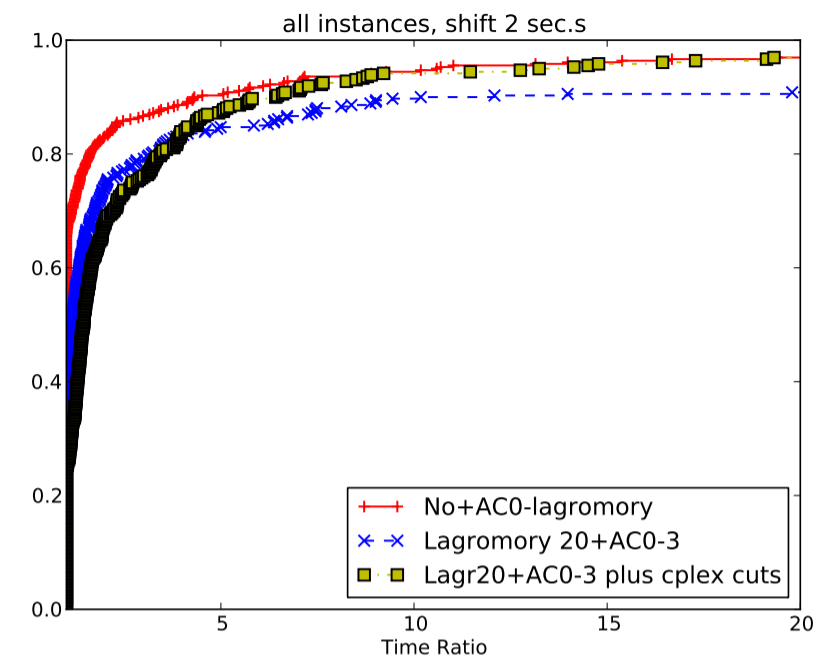
\includegraphics[scale=0.5]{Images/profile_out}\\ 
\end{center} 
\end{figure}
}
\end{itemize}


%Bibliografia
\addcontentsline{toc}{chapter}{Bibliografia}
\bibliographystyle{plain}
\renewcommand{\bibname}{Bibliografia}
\bibliography{Chapters/biblio}

\end{document}